
%%%%%%%%%%%%%%%%%%%%%%% file typeinst.tex %%%%%%%%%%%%%%%%%%%%%%%%%
%
% This is the LaTeX source for the instructions to authors using
% the LaTeX document class 'llncs.cls' for contributions to
% the Lecture Notes in Computer Sciences series.
% http://www.springer.com/lncs       Springer Heidelberg 2006/05/04
%
% It may be used as a template for your own input - copy it
% to a new file with a new name and use it as the basis
% for your article.
%
% NB: the document class 'llncs' has its own and detailed documentation, see
% ftp://ftp.springer.de/data/pubftp/pub/tex/latex/llncs/latex2e/llncsdoc.pdf
%
%%%%%%%%%%%%%%%%%%%%%%%%%%%%%%%%%%%%%%%%%%%%%%%%%%%%%%%%%%%%%%%%%%%


\documentclass[runningheads,a4paper]{llncs}

\usepackage{amssymb}
\setcounter{tocdepth}{3}
\usepackage{graphicx}

\usepackage{url}
\urldef{\mailsa}\path|{dedek, eckhardt, vojtas}@ksi.mff.cuni.cz|
\urldef{\mailsb}\path|anna.kramer, leonie.kunz, christine.reiss, nicole.sator,|
\urldef{\mailsc}\path|erika.siebert-cole, peter.strasser, lncs}@springer.com|    
\newcommand{\keywords}[1]{\par\addvspace\baselineskip
\noindent\keywordname\enspace\ignorespaces#1}

\begin{document}

\mainmatter  % start of an individual contribution

% first the title is needed
\title{Annotating Web for Users}

% a short form should be given in case it is too long for the running head
\titlerunning{Annotating Web for Users}

% the name(s) of the author(s) follow(s) next
%
% NB: Chinese authors should write their first names(s) in front of
% their surnames. This ensures that the names appear correctly in
% the running heads and the author index.
%
\author{Jan D\v{e}dek \and Alan Eckhardt \and Peter Vojt\'{a}\v{s}}
%
\authorrunning{D\v{e}dek, Eckhardt, Vojt\'{a}\v{s}}
% (feature abused for this document to repeat the title also on left hand pages)

% the affiliations are given next; don't give your e-mail address
% unless you accept that it will be published
\institute{Department of Software Engineering, Faculty of Mathematics and Physics\\
Charles University in Prague, Czech Republic \\
\mailsa\\
%\mailsb\\
%\mailsc\\
%\url{http://www.ksi.mff.cuni.cz/}
}

%
% NB: a more complex sample for affiliations and the mapping to the
% corresponding authors can be found in the file "llncs.dem"
% (search for the string "\mainmatter" where a contribution starts).
% "llncs.dem" accompanies the document class "llncs.cls".
%

\toctitle{Annotating Web for Users}
\tocauthor{D\v{e}dek, Eckhardt, Vojt\'{a}\v{s}}
\maketitle


\begin{abstract}
Annotating Web for Users
\keywords{Semantic Annotation, User Preferences, Machine Learning}
\end{abstract}


\section{Semantic Annotation}
Semantic annotation (SA) is considered to be one of the most important elements in the evolution of the Semantic Web. It can provide great help in the process of data and information integration and it could also be a basis for intelligent search and navigation. Users can easily get all available information to given topic and see or directly navigate to relevant related facts which can be spread over the whole (Semantic) Web.

\subsection{Web Information Extraction}
Web information extraction \cite{biblio:WebDataMining} is often able to extract valuable data. We would like to couple the extraction process with the consecutive semantic annotation (initially human trained; later it should operate automatically). Our idea is to split the extraction process in two parts - domain independent and domain dependent. 


Our first approach for domain independent intermediate information extraction and semantic annotation is to use the structural similarity in web pages containing large number of table cells and for each cell a link to detailed pages. This is often presented in web shops and on pages that presents more than one object (product offer). Each object is presented in a similar way and this fact can be exploited \cite{biblio:EcHoUncertaintyIssues2008}.


Our second approach for Web information extraction is targeted to textual pages. It is based on deep linguistic analysis (DLA) produced by Czech linguistics and NLP tools. We use a chain of linguistic analyzers prom the PDT and TectoMT projects that processes the text presented on a web page and produces linguistic (syntactic) trees corresponding with particular sentences. These trees serve as a basis of our semantic extraction. We use a machine learning method based on Inductive Logic Programming (ILP). The combination of DLA and ILP have several benefits: no need of manual selection of learning features, the learning procedure is capable to select relevant parts itself and to construct linguistic extraction rules, which can be easily visualized, understood and adapted by human \cite{biblio:DedekISWC2010}. 

\subsection{Collaborative Approach}
Although automated and machine learning based methods for Information Extraction and Semantic Annotation can significantly reduce the amount of necessary human work, it is clear that it will be never possible avoid it completely. Therefore it is useful to heave a fancy tool that would be attractive to human users providing them an easy way of doing manual semantic annotation \cite{biblio:FiserMaster}. Thus these users could benefit from having the content of their interest semantically annotated with as low cost as possible. To reduce the costs, which means to reduce the amount of manual annotations per user, we plan to develop a community site with a semantic repository \cite{biblio:LasekWWW} where annotation work can be shared amongst users and assisted by automated tools.

\section{User preferences on the web}
User preference learning is also loosely connected to Semantic web. It is not the core aspect, but without knowing the users needs, the semantic web wouldn't be able to improve user experience. We are investigating the area of preference learning. Since this area consists of many diverse topics, we currently concentrate on content based learning from user's ratings, but the focus shifts towards interpreting user behaviour. Our main motivation is preference learning. The main focus is to learn the preference of one specific user - we are not interested in "the average user".

 
We are working with the assumption of having annotated data in the database or other repository. Semantic web initiative enables the annotation of data. Annotated data allows us to use the attributes of the objects that may be difficult to find. The attributes may be stored on different web sites; the pages may have complicated structure, etc. 

\begin{figure}
	\centering
		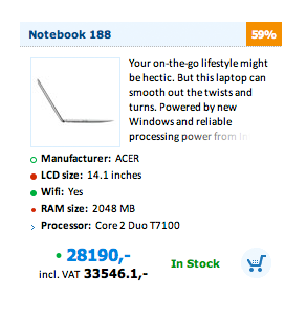
\includegraphics{imgVaclav}
	\caption{Attribute visualisation in the web shop interface}
	\label{img:Vaclav}
\end{figure}


The paradigm of content based learning is to understand what properties an object should have in order to be preferred. Knowing which attribute values are desirable is important for many reasons. Being able to visualise the object and to emphasise those desired properties is the user interface part \cite{biblio:FiserMaster} (see the picture \ref{img:Vaclav}). Another advantage is the use of preferences in the database aspect, top-k query answering and indexing techniques \cite{Fagin:2001:OAA:375551.375567}. 


Our approach is divided into two steps - criteria for each attribute are learnt during the first step, the preference degrees of attributes are aggregated into the overall preference of the whole object during the second step. The first step transforms attributes from ``price'' to ``cheap'' and ``weight'' to ``light'' (or ``heavy'', which depends on the user). The second step then computes the overall preference of the object, based on the satisfaction of the (learnt) criteria.


There are various problems addressed. The first kind of problem comes from the preference nature - the sample rated by the user on the web is often very small (up to 50 objects) and the rating is given on a small set of rating, usually 1,2,3,4,5. Another kind of problem arises from the need to have a transparent user preference model, which will allow it to be used in other components of the system - indexing, query processing.


The most recent area is user behaviour mining. This area is much more difficult than using user ratings to assess his/her preferences, because behaviour contains the preferences only implicitly and we cannot be sure whether they are contained at all. However, our preliminary experiments in \cite{biblio:Peska} have shown that it is possible even on real world web shops. Much more investigation is needed in this area for better acquaintance with the subject. 




\subsection*{Acknowledgments}
This work was partially supported by Czech projects: GACR P202/10/0761, GACR-201/09/H057, GAUK 31009 and MSM-0021620838.

\bibliographystyle{splncs03}
\bibliography{DedEckVoj_SIIS_Warsaw_Lux}


\end{document}
